\documentclass{article}
\usepackage{ctex}                               %显示中文,更改字体
\usepackage{setspace}                           %调整页行距
\usepackage{geometry}                           %设置页边距
\usepackage{booktabs}                           %制作三线表
\usepackage{graphicx}                           %插入图片
\usepackage{indentfirst}                        %首行缩进
\usepackage{float}                              %图片位置
\usepackage{makecell}                           %处理表格
\usepackage{amsmath}                            %公式处理
\usepackage{amssymb}                            %公式处理
\usepackage{titlesec}                           %标题处理
\usepackage{tikz}                               %带圈数字
\usepackage{enumerate}                          %编号排版
\usepackage{appendix}                           %附录排版
\usepackage{listings}                           %插入代码
\usepackage{xcolor}                             %代码颜色
\newcommand*{\circled}[1]{\lower.7ex\hbox{\tikz\draw (0pt, 0pt) circle (.45em) node {\makebox[1em][c]{\small #1}};}}
%由于自带效果不好,自定义带圈的数字样式
\title{\zihao{-2}无线可充电传感器网络充电路线规划\vspace{-2em}}
%文章标题 且拉进与正文距离 默认 三号
\date{}     %取消时间显示
\author{}   %取消作者显示
\renewcommand{\baselinestretch}{1.5}
%调整行距为1.5倍标准行距
\renewcommand\refname{\ }           
%把"reference"改成"参考文献"
\renewcommand{\abstractname}{\zihao{3} 摘\ 要\\\vspace{1em}}
%把“abstract”改成“摘要” 且拉开与正文距离
\geometry{left=3.18cm,right=3.18cm,top=2.54cm,bottom=2.54cm}
%设置页边距,此处参考word默认间距
\titleformat*{\section}{\zihao{3}\bfseries}
\titleformat*{\subsection}{\zihao{-3}\bfseries}
\titleformat*{\subsubsection}{\zihao{4}\bfseries}
%三级标题均改变字号,黑体
\titleformat{\paragraph}
{\normalfont\zihao{-4}\bfseries}{\theparagraph}{1em}{}
\titlespacing*{\paragraph}
{0pt}{3.25ex plus 1ex minus .2ex}{1.5ex plus .2ex}
%设置四级标题 用\paragraph实现
\setcounter{secnumdepth}{4}
%改变章节编号深度,使得四级标题编号自动生成,如需目录章节深度则使用tocdepth
\lstset{
  language=Matlab,  %代码语言使用的是matlab
  keywordstyle=\color{blue!90}\bfseries, %代码关键字的颜色为蓝色,粗体
  commentstyle=\color{red!20!green!90}\textit,    % 设置代码注释的颜色为绿色
  showstringspaces=false,%不显示代码字符串中间的空格标记
  stringstyle=\ttfamily, % 代码字符串的特殊格式
  breaklines=true, %对过长的代码自动换行
  extendedchars=false,  %解决代码跨页时,章节标题,页眉等汉字不显示的问题
  texcl=true}
\lstset{breaklines}%自动将长的代码行换行排版
\lstset{extendedchars=false}%解决代码跨页时,章节标题,页眉等汉字不显示的问题
\begin{document}
\setlength{\parindent}{2em}         
%首行缩进两字符
\maketitle                                                  %生成文章题目,作者,时间
\thispagestyle{empty}                                       %本页不生成页码
\begin{abstract}                                            %摘要 开始
{\zihao{-4}                                                 %摘要 小四
无线可充电传感器网络在无线传感网络WSN中起到提供能量的作用,其内部的充电线路以及传感器的电池容量会影响充电效率以及能源损耗。对于给定参数的传感器,本文通过建立数学模型,研究了使得充电网络能源消耗最小的充电路线和能使整个系统一直正常工作的传感器电池容量。

对于问题一,首先根据附件的传感器的经纬度位置,计算每个传感器之间的实际距离,然后将问题转变为求从数据中心出发,依次经过每一个传感器然后回到数据中心的这一路线的最短距离。然后根据题目要求建立了目标函数,其中以第i个节点是否到达第j个节点作为决策变量,以从数据中心出发遍历每一个节点然后回到数据中心的最小距离作为目标函数,其中保证每一个节点有且只经过一次来建立数学模型。然后通过遗传算法来解决该问题,在解决问题的过程中,进行了几次优化,进行了几次搜索,得到的结果从14143m→13262m→13060m→11895m,所以得到了最优路线以及最短路程。

对于问题二,移动充电器的工作原理是从数据中心出发,行驶一段路程后到达传感器并给其充电,依次给29个传感器充完电后再返回数据中心,由于题设要求需一直保持工作状态,所以需要考虑两个过程:一是返回到数据中心;二是再次为传感器充电,需要保证在这两个过程完成的时候传感器的电量仍然大于阈值即传感器能正常工作。这里通过分析传感器消耗能量的时间分为两个部分——为传感器充满电量所消耗的时间和充电器到达传感器消耗的时间,然后以传感器所要消耗的能量为目标函数,所求解的电池容量为这一目标函数加上阈值。

\setlength{\baselineskip}{20pt}     对于问题三,与问题一、二不同之处在于,移动充电器的数量从1个增至4个,在这个改变之上再求解出移动充电器的行驶路线和传感器的电池容量。移动充电器的数量增加,则线路的规划即可视为MTSP问题,同样运用遗传算法来解决。电池容量的求解也与第二问类似,可以视为把一条路线划分成4条互相独立的路线,再结合第二问的公式,即可解出。\\

\noindent \textbf{关键词:}无线传感网络\quad MTSP问题\quad 遗传算法\quad 数值解法\quad MATLAB软件
%局部取消缩进
}
\thispagestyle{empty}
%本页不生成页码 摘要写的太多 多了一页
\end{abstract}                                              %摘要 结束
\newpage                                                    %换页
\setcounter{page}{1}                                        %文章页码从1开始重新编排
\section{问题重述}                                          %换页
\subsection{背景介绍}
\zihao{-4}                                                  %正文小四
随着物联网的快速发展,无线传感器网络WSN(Wireless Sensor Network)在生活中的应用也越来越广泛。无线传感器网络中包括若干传感器(Sensors)以及一个数据中心(Data Center)。传感器从环境中收集信息后每隔一段时间将收集到的信息发送到数据中心。数据中心对数据进行分析并回传控制信息。

影响WSN生命周期最重要的一个因素是能量。想要让WSN能够持续不断地运转,就必须持续为WSN提供能量。提供能量的方式之一是能量收集(Energy Harvesting),通过利用太阳能或风能等环境能源让传感器自行从环境中汲取能量以维持其运作。然而这种方式提供的能量不但不稳定,而且太过于依赖环境,一旦环境达不到条件,WSN无法从环境中汲取能量自然也就无法运转。提供能量的另外一种方式是电池供电,并利用移动充电器定期为传感器的电池补充能量,从而源源不断地为WSN提供稳定的能量使其正常运转。通过这种方式供电的网络也被称为无线可充电传感器网络WRSN(wireless Rechargeable Sensor Network)。
\subsection{问题描述}
无线可充电传感器网络包括三个部分:一个数据中心DC(Data Center)、若干传感器(Sensors)、一个或多个移动充电器MC(Mobile Charger)。

数据中心和若干传感器分布在一个二维空间中,如下图所示(虚线箭头表示数据中心与传感器之间、传感器与传感器之间均存在一条路径互相连通;实线箭头表示MC的充电路线)。

\begin{figure}[H]%先尝试能否将照片放在原处(here),如果不能,那么放在页面底部(bottom),最后尝试放在顶部(top) 都不可以采用H强制放在原位
    \centering
    
\includegraphics[scale=0.5]{1.jpg}
    \caption{数据中心和传感器分布图}
\end{figure}

在该系统中,传感器从环境中收集信息并将收集到的信息传递给数据中心。当一个传感器的电量低于一个阈值时便无法进行正常的信息采集工作,为了让WRSN正常运转,移动充电器需要定期为传感器进行充电以避免其电量低于阈值。

移动充电器从数据中心出发,以固定的速度依次经过每个传感器,在每个传感器处停留一段时间并以固定的充电速率为传感器充电,直到为所有传感器充电完成之后返回数据中心。每个传感器都有特定的能量消耗速率,以及固定的电池容量。移动充电器的能量消耗主要有两个方面:一是为传感器节点充电所导致的正常的能量消耗;另外一方面则是移动充电器在去为传感器充电的路上的能量消耗。为了减小移动充电器在路上的能量消耗,需要合理地规划移动充电器的充电路线。请考虑以下问题:
\begin{enumerate}[\indent 1.]
\item 若给出每个节点的经纬度(见附件1),请考虑当只派出一个移动充电器时,如何规划移动充电器的充电路线才能最小化移动充电器在路上的能量消耗。

\item 若给出每个节点的经纬度、每个节点的能量消耗速率(见附件2),并假设传感器的电量只有在高于f(mA)时才能正常工作,移动充电器的移动速度为v(m/s)、移动充电器的充电速率为r(mA/s),在只派出一个移动充电器的情况下,若采用问题1)规划出来的充电路线,每个传感器的电池的容量应至少是多大才能保证整个系统一直正常运行(即系统中每个传感器的电量都不会低于f(mA))?

\item 若给出每个节点的经纬度、每个节点的能量消耗速率(同见附件2),并假设传感器的电量只有在高于f(mA)时才能正常工作,移动充电器的移动速度为v(m/s)、移动充电器的充电速率为r(mA/s),但为了提高充电效率,同时派出4个移动充电器进行充电,在这种情况下应该如何规划移动充电器的充电路线以最小化所有移动充电器在路上的总的能量消耗?每个传感器的电池的容量应至少是多大才能保证整个系统一直正常运行?
\end{enumerate}
\newpage
\section{问题分析}
\subsection{模型的分析}
\subsubsection{问题一}
我们需要减少充电器在路上的能量消耗,由于充电过程中节点的能量消耗是固定的,我们只需要使得充电路线最短,便能够最小化充电路上的能量消耗,所以我们需要求得从数据中心出发,依次经过每一个节点,然后返回数据中心的最短路线,可以将此问题看成为哈密顿问题或者是旅行商问题;
\subsubsection{问题二}
移动充电器是沿着问题一得出的路线进行行驶,从第1个传感器开始充电,直至29个传感器皆完成充电任务,最终返回数据中心。因要保证整个系统一直正常运行,所以移动充电器不断进行循环充电。针对这个问题,我们从传感器第一次充电到第二次充电这个过程分析。将这个过程分为两个步骤,第一步为移动充电器第一次给传感器充电并返回数据中心;第二步为移动充电器从数据中心出发到给传感器第二次充电。通过分析在这两个步骤中所花费的时间和传感器消耗的电量,来建立模型求解出传感器的最低电池容量。
\subsubsection{问题三}
由于问题三是在问题一和问题二的基础上进行的优化,这里所要考虑的问题没有发生变化,只是由一个充电器增加到了四个充电器,即由单旅行商问题演变成了多旅行商问题,我们仍然是要求出四个充电线路的最短路径之和来使得充电路上的能量消耗最小,在这一基础上,建立模型求解传感器的最低电池容量。
\subsection{模型的准备及相关流程}
这里我们所要运用到的模型是旅行商问题,所要采用的算法是遗传算法,所以在这里我们对旅行商问题和遗传算法进行简单的介绍。
\subsubsection{旅行商问题}
旅行商问题是寻找n个城市的最短(闭)环游,使得在回到起点之前,每个城市均被访问且只访问一次,它的英文名称为TSP\cite{ref1} ,而多旅行商问题便是旅行商问题(TSP)的拓展,被称为MTSP问题,它是给定一个中心城市和n个访问城市,将访问城市分配给m个旅行商,每个旅行商从中心城市出发巡游若干访问城市后回到中心城市,要使旅行商经过的总路程尽量小且其中最长环路的长度尽量小\cite{ref2}。
\subsubsection{遗传算法}
遗传算法是基于生物遗传进化思想的一种优化方法,因此遗传算法与数学规划类优化方法在原理,实现手段等方面有着明显的差别。遗传算法包含许多名词,这里做一个简单的介绍:

个体:用来模拟生物染色体的一定数目的二进制位串;

群体:一定数量的个体组成的集合;

基因模式:二进制位串表示的个体中,某一或某一些位置上具有相似性的个体组成的集合;

模式阶次:基因模式中包含相似位置的数目;

模式定义长度:基因模式中相似位间相距的最大距离

适应度:以数值方式来描述个体优劣程度的指标;

平均适应度:若干个个体的适应度值的算术平均值;

繁殖:由一代群体繁衍产生另一代群体的方式总称;

选择:在上一代群体中按照某些指标挑选参与繁殖下一代群体的一定数量的个体;

杂交:对优选后的父代个体进行基因模式的重组而产生后代个体的繁殖机制;

突变;模拟生物在自然的遗传进化环境中由于各种偶然因素引起的基因模式突然改变的个体繁殖方式\cite{ref3}。

以下是遗传算法的流程:


\newpage                                                    %换页
\section{模型假设与约定}
\begin{enumerate}
\item 在充电过程中只考虑传感器节点消耗电量和充电路程消耗电量;
\item 在充电路程中所消耗的能量与充电路程成正比,不考虑其他因素的影响;
\item 传感器在第一次充电前电量为0且充电后是满电状态;
\item 假设移动充电器在数据中心不停留;
\item 文中所说第i个传感器指沿线路经过的第i个,并非传感器i
\end{enumerate}
\vspace{4em}
\section{符号说明与名词定义}
\vspace{4ex}                %空行 距离为当前文字大小下x
\begin{center}              %三线图 
    \begin{tabular}{cccc}
        \toprule
        符号    & 名词  & 符号  & 名词\\
        \midrule
        E$_0$  & 消耗的总能量        & r    & 移动充电器的充电速率    \\

        E$_1$  & 传感器节点充电所消耗的能量 & c    & 传感器能量消耗速率     \\

        E$_2$  & 传感器充电路上消耗的能量  & a    & 传感器电池容量       \\

        d   & 单充电器的移动充电器总路程 & q    & 传感器消耗的电量      \\

        R   & 地球半径          & t    & 每一轮消耗的时间      \\

        d$\rm _{ij}$ & 两个传感器之间的距离    & Q    & 总消耗的电量        \\

        x$\rm _{ij}$ & 单充电器决策变量      & B    & 四个充电器的集合      \\

        A   & 30个点的集合       & x$\rm _{ijk}$ & 多充电器的决策变量     \\

        f   & 传感器电量阈值       & d$_1$   & 多充电器的移动充电器总路程 \\

        v   & 移动充电器的移动速度    &      &   \\
        \bottomrule
    \end{tabular}
\end{center}

\newpage                                                    %换页
\section{模型的建立与求解}
\subsection{问题一}
对于问题一,我们需要求解当只派出一个移动充电器时,规划移动充电器的充电路线使得移动充电器在路上的能量消耗最小。\\
\vspace{0.5ex}
\begin{figure}[hbt]
	\begin{minipage}[t]{0.5\textwidth}
		\centering
		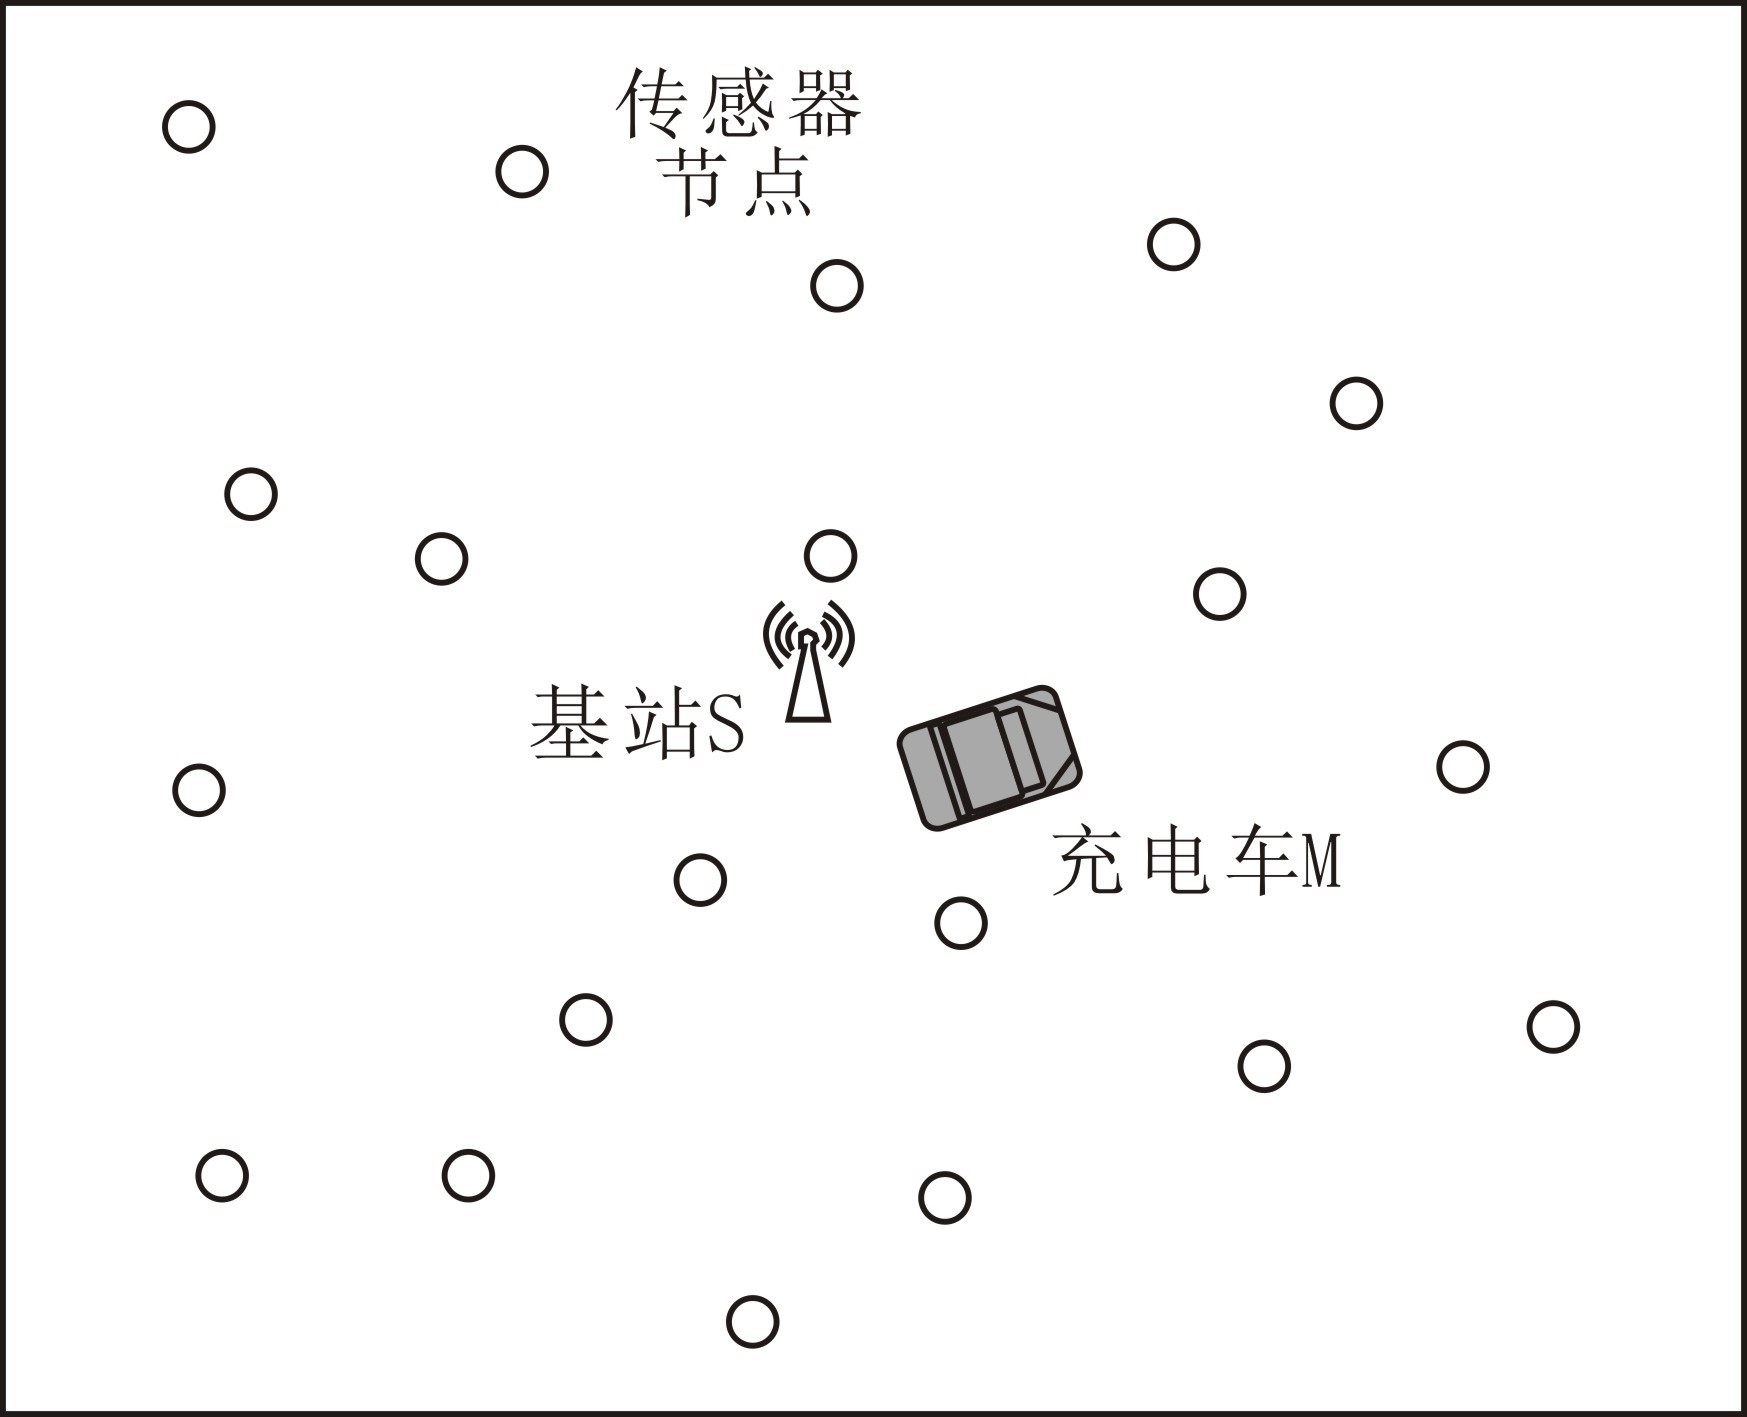
\includegraphics[scale=0.5]{3.jpg}
		\caption{单充电器无线充电网络}
	\end{minipage}
	\qquad
	\begin{minipage}[t]{0.5\textwidth}
		\centering
		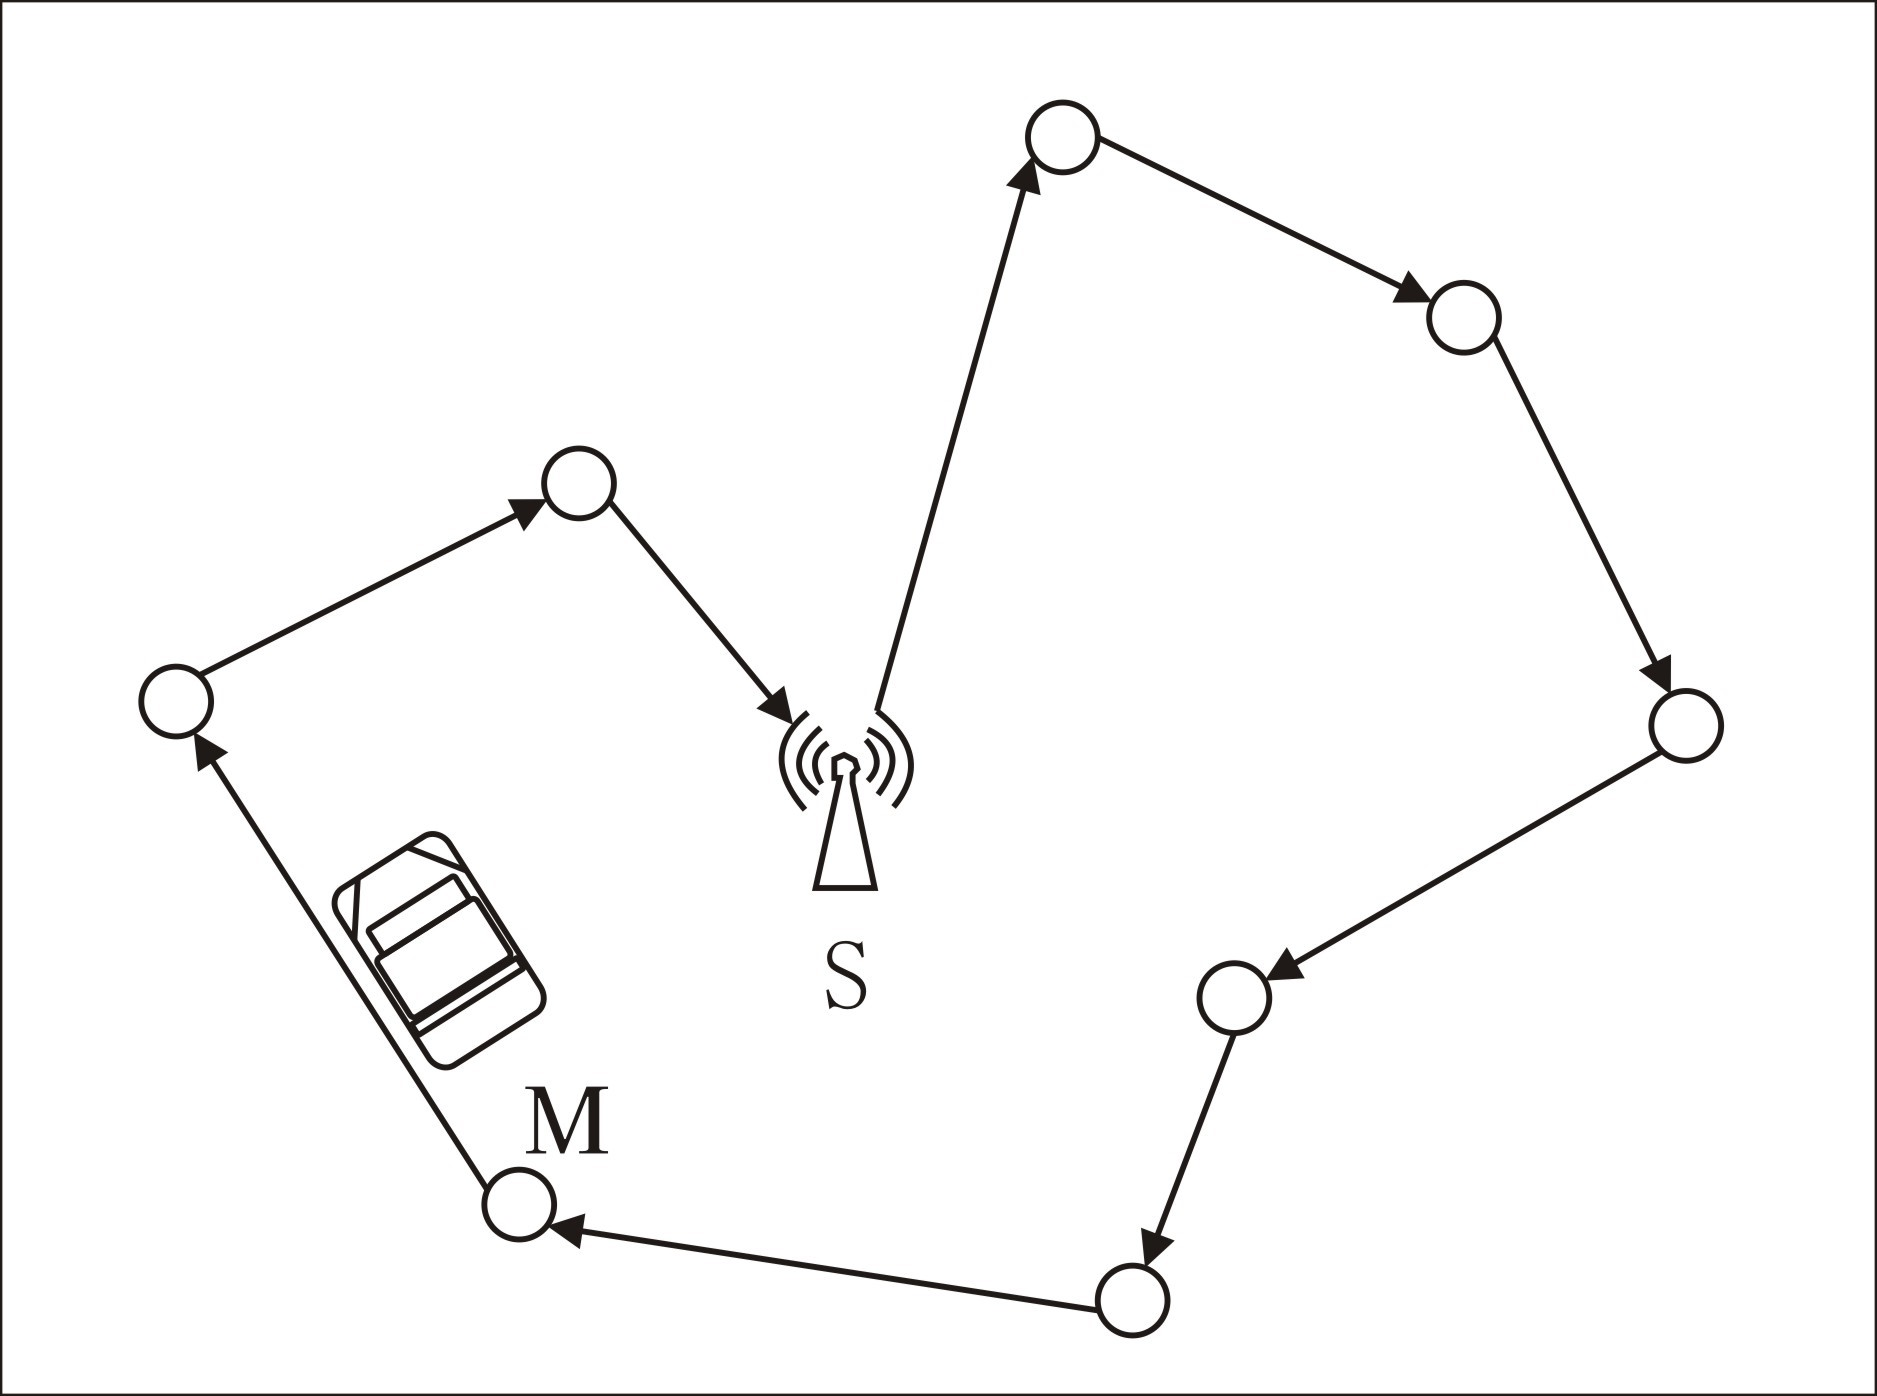
\includegraphics[scale=0.5]{4.jpg}
		\caption{单充电器充电线路模型}
	\end{minipage}
\end{figure}
\vspace{0.5ex}

这里我们由题目可以了解到:移动充电器在路上的能量消耗分为两部分——传感器节点充电所导致的正常的能量消耗和移动充电器在去为传感器充电的路上的能量消耗。设E$_0$为消耗的能量,E$_1$为传感器节点充电所消耗的能量,E$_2$为传感器充电路上的能量消耗,则有:
\begin{equation}
    E_0 = E_1 + E_2     %此处存疑,不理解为什么行间公式就可以不用$
    \tag{1}             %初步理解为由于公式使用$会直接结束公式
\end{equation}      %使用tag自定义编号

在这个过程中,由于E$_1$是由充电节点的性质和传感器充电时间所决定,所以我们可以将E1视作固定的,为了使E$_0$最小,我们需要使E$_2$最小,假设充电路程为d,E$_2$与d的相关系数为$\alpha$,则有:
\begin{equation}
    E_2 = \alpha \cdot d   %此处不使用$原因如上
    \tag{2}             
\end{equation}      

所以要使得E2最小,就是要求得充电路程d最小;


\subsubsection{求解20个坐标的实际距离}
要求得充电路程最小,我们可以将这一个问题转变为求最短路径问题,首先我们需要求出30个坐标之间的实际距离\cite{ref4}:

附件一给出的坐标是地理坐标(经度和纬度),我们需要求的是两点的实际距离。设A,B两点的地理坐标分别是(x$_1$,y$_1$),(x$_2$,y$_2$),过A,B两点的大圆的劣弧长即为两点的实际距离。以地心为坐标原点O,以赤道平面为XOY平面,以0度经纬圈所在的平面为XOZ平面建立三维直角坐标系,则A,B两点的直角坐标为分别:
\begin{gather}    %使用gather多行公式加编号
    \mathrm {A\left(R \cdot \cos x_1 \cdot \cos y_1, R \cdot \sin x_1 \cdot \cos y_1, R \cdot \sin y_1\right)} \tag{3} \\
    \mathrm {B\left(R \cdot \cos x_2 \cdot \cos y_2, R \cdot \sin x_2 \cdot \cos y_2, R \cdot \sin y_2\right)} \tag{4}            
\end{gather}    % \left \right 保证高度

其中R=6370为地球半径

A,B两点的实际距离为:
\begin{equation}
    \mathrm {\left.d_0 = Rarccos {\left(\frac{\overrightarrow{O A} \cdot \overrightarrow{O B}}{|\overrightarrow{O A}| \cdot|\overrightarrow{O B}|}\right.}\right)}
    \tag{5}
\end{equation}      %\frac{}{} \overrightarrow 向量

化简得
\begin{equation}
    \mathrm{ d_0 = Rarccos \left[\cos \left(x_1 - x_2\right) \cdot \cos y_1 \cdot \cos y_2 + s iny_1 \cdot s iny_2\right]}
    \tag{6}
\end{equation}


根据附件一的数据使用MATLAB软件求出各点之间的实际距离结果见附件。

\subsubsection{数学模型的建立}
该模型可以视作旅行商问题,旅行商问题的数学模型为:假设有n个(n为有限个正自然数)城市集合,求解一个城市的序列I使得从一个城市出发,遍历所有城市后又回到原城市的总路程最小。这里我们设这30个点的集合为A= $\left\{1,2,…,i,j,…,30\right\}$;其中两城市之间的距离记为{$ \rm d_{ij}$} $(1 \leqslant i,j \leqslant 30)$ ,我们设置决策变量为{$ \rm x_{ij}$},定义为:
$$
\rm {x_{ij}=\left\{
    \begin{array}{l}
        \text{1路线从i到达j} \\
        \text{0路线没有从i到达j}
    \end{array}
\right.}
$$      %此处不需要编号所以行间公式选择使用$${...}$$

所以求解总路程的目标函数为:
\begin{equation}
    \mathrm{d=\min \sum_{i \neq j} d_{i j} \cdot x_{i j}}
    \tag{7}
\end{equation}

约束条件需要满足每一个点进去和出来都是一次,所以约束条件为:
\begin{gather}    %使用gather多行公式加编号
    \mathrm {\sum_{i \neq j}^{n} x_{i j}=1 \quad \mathrm{i}=1,2, \cdots, 30} \tag{8}\\
    \mathrm {\sum_{j=1}^{n} x_{i j}=\underline{1} \quad \mathrm{j}=1,2, \cdots, 30} \tag{9}           
\end{gather}    

需要保证走过的所有路径没有回路,则需要满足:
\begin{gather}    %使用gather多行公式加编号
    \mathrm {\sum_{i, j \in A} x_{i j} \leqslant|A|-1, \quad 2 \leqslant |A| \leqslant 28,\quad A \subset \{1,2, \cdots, 30\}} \tag{10}\\
    \mathrm {x_{i , j} \in\{0,1\}, \quad i = j =1,2, \cdots, 30 ; \mathrm{i} \neq j} \tag{11}      
\end{gather} 

以上保证了所得到的总路径最小,并且每个传感器有且只经过了一次,走过的路径没有回路。

\subsubsection{模型的求解}
分析决定采用遗传算法解决问题。根据已有目标函数映射适应度函数:
$$\mathrm{d=\min \sum_{i \neq j} d_{i j} \cdot x_{i j}}$$

\paragraph{编码策略}
采用十进制编码,用随机数列$\omega_1$ $\omega_2$ $\omega_3$ … $\omega_{30}$作为染色体,其中0< $\omega_i$ <1(i=2,3,…,30), $\omega_1$ = 0, $\omega_{30}$ = 1;每一个随机序列都和种群中的一个个个体相对应,例如一个9城市问题的一个染色体为:
$$\left[0.23,0.82,0.45,0.74,0.87,0.11,0.56,0.69,0.78\right]$$
其中编码位置i代表城市i,位置i的随机数表示城市i在充电中的顺序,我们将这些随机数按升序排列得到如下顺序:
$$6-1-3-7-8-4-9-2-5$$

\paragraph{初始种群}
由于传感器数量不多,所以初始种群随机产生,不做初步优化

\paragraph{参数选择}
初始参数我们按照基本参数设定为:

种群大小:inn = 30

最大代数:gnMax = 500

交叉率:crossProb = 0.9

变异率:muteProb = 0.1

第一次得到的结果和搜索过程如下:


显然,此时的结果图中,有明显的交叉路径,在寻求最优解的过程中,变异次数略小;而在搜索过程中,我们所得的结果并没有得到长时间,即多代数的验证,所以将参数调整为:

种群大小:inn = 30

最大代数:gnMax = 1000

交叉率:crossProb = 0.9

变异率:muteProb = 0.15

此时得出的结果和搜索过程为:


可以明显看出结果显然不是最优解,为保证种群的充分进化,交叉概率我们可以选择为1,得出如下结果: 



可以看出,由于交叉概率调整为1,导致的代数和变异概率需要进一步调整,结果如下:


结果趋于稳定,所以选择如上参数
\paragraph{选择}
采用确定性的选择策略,也就是说选择目标函数值最小的inn个体进化到下一代,这样可以保证父代的优良特性被保存下来。
\subsubsection{实验结果}
由此可知,使得充电线路上消耗最小的充电路线为:

\vspace{2ex}
\noindent 数据中心$\Rightarrow$节点2\;$\Rightarrow$节点1\;$\Rightarrow$节点9\;$\Rightarrow$节点7\;$\Rightarrow$节点6\;$\Rightarrow$节点14\;$\Rightarrow$节点11\;$\Rightarrow$节点8\;$\Rightarrow$节点12\;$\Rightarrow$节点15\;$\Rightarrow$节点27\;$\Rightarrow$节点16\;$\Rightarrow$节点13\;$\Rightarrow$节点10\;$\Rightarrow$节点5\;$\Rightarrow$节点3\;$\Rightarrow$节点4\;$\Rightarrow$节点28\;$\Rightarrow$节点24\;$\Rightarrow$节点23\;$\Rightarrow$节点22\;$\Rightarrow$节点21$\Rightarrow$节点29\;$\Rightarrow$节点19\;$\Rightarrow$节点26\;$\Rightarrow$节点25\;$\Rightarrow$节点18\;$\Rightarrow$节点20\;$\Rightarrow$节点17\;$\Rightarrow$数据中心
\vspace{2ex}

其中求出来的总路程d=11895m

\subsection{问题二}
对于问题二,因需保证整个系统一直正常运行,所以每个传感器的电量总是要高于阈值,即在下一次充电前电量不低于f (mA)。在第一轮充电时,传感器电量从0充至满电量,在后续的每轮充电中,传感器电量均从f充至满电。所以我们通过分析移动充电器对于传感器的第一次充电和第二次充电即可。
\subsubsection{第一轮充电过程}
分析移动充电器从数据中心出发充完电后再返回到数据中心这一过程内,所需的时间和传感器消耗的电量\cite{ref5}。


先分析第1个传感器,当其充满电后,移动充电器返回到数据中心需经过29条路和28个传感器,则在路上所耗费时间为:
\begin{equation}
    \mathrm{t_{\text {路} 1}=\frac{d_{2}+d_{3}+\cdots+d_{30}}{v}}
    \tag{12}
\end{equation}

在给其他传感器充电所耗费的时间为:
\begin{equation}
    \mathrm{{\text {传} 1}=\frac{a_{2}+a_{3}+\cdots+a_{29}}{r}}
    \tag{13}
\end{equation}

所以总消耗时间为:
$$\mathrm{t_1=t_{\text {传1}}+t_{\text {路1}}}$$

在这段时间内传感器1消耗的电量为:
$$\mathrm{q_1=c_1 t_1}$$

第1个传感器在这段过程里的时间和消耗电量已经分析出来了,剩余的传感器以此类推进行分析,如下表格所示:
\vspace{1ex}
\begin{table}[h]
    \begin{center} 
        \begin{tabular}{|p{1.5cm}<{\centering}|p{1.5cm}<{\centering}|p{1.5cm}<{\centering}|c|c|p{2cm}<{\centering}|}
            \hline
            \makecell*[c]{第i个\\传感器} & \makecell*[c]{经过路\\线条数} & \makecell*[c]{经过传感\\器的个数}  & 在路程上所耗费的时间            & 其余传感器充电时间             & \makecell*[c]{在总时间内\\消耗的电量}  \\ 
            \hline
            1      & 29     & 28       & $\frac{d_{2}+d_{3}+\cdots+d_{30}}{v}$ & $\frac{a_{2}+a_{3}+\cdots+a_{29}}{r}$  &  $\makecell*[c]{c_1 t_1}$   \\ 
            \hline
            2      & 28     & 27       & $\frac{d_{3}+d_{4}+\cdots+d_{30}}{v}$ & $\frac{a_{3}+a_{4}+\cdots+a_{29}}{r}$  &  $\makecell*[c]{c_2 t_2}$  \\ 
            \hline
            \multicolumn{6}{|c|}{$\cdots \cdots$}                                                                 \\ 
            \hline
            29     & 1      & 0        & $\frac{d_{30}}{v}$     &  0  &  $\makecell*[c]{c_{29} t_{29}}$ \\
            \hline
        \end{tabular}
    \end{center}
\caption{传感器第一轮耗费时间与电量}
\end{table}

第一轮中第i个传感器消耗的电量:($a_{30}$=0 )
\begin{equation}
    \mathrm{q_i=\left(\frac{\sum_{i+1}^{30} d_{i+1}}{v}+\frac{\sum_{i+1}^{29} a_{i+1}}{r}\right) * c_i=c_i t_i}
    \tag{14}
\end{equation}

\subsubsection{第二轮充电过程}
分析在第二轮充电中,移动充电器从数据中心出发到给各传感器充电这一过程内,所需的时间和传感器消耗的电量,其过程与第一轮相似,同样只详细分析第1个:

移动充电器从数据中心到第1个传感器,需经过1条路和0个传感器,则在路上所耗费时间为:
\begin{equation}
    \mathrm{t_{\text {路1}}^{\prime}=\frac{d_{1}}{v}}
    \tag{15}
\end{equation}

在给其他传感器充电所耗费的时间为:
\begin{equation}
    \mathrm{t_{\text {传1}}^{\prime}=0}
    \tag{16}
\end{equation}

所以总消耗时间为:
\begin{equation}
    \mathrm{t_{1}^{\prime}=t_{\text {路1}}^{\prime}}
    \tag{17}
\end{equation}

在这段时间内传感器1消耗的电量为:
\begin{equation}
    \mathrm{q_{1}^{\prime}=c_{1}^{\prime} t_{1}^{\prime}}
    \tag{18}
\end{equation}

其余传感器的数据如下表所示:
\vspace{1ex}
\begin{table}[h]
    \begin{center} 
        \begin{tabular}{|p{1.5cm}<{\centering}|p{1.5cm}<{\centering}|p{1.5cm}<{\centering}|c|c|p{2cm}<{\centering}|}
        \hline
        \makecell*[c]{第i个\\传感器} & \makecell*[c]{经过路\\线条数} & \makecell*[c]{经过传感\\器的个数}  & 在路程上所耗费的时间            & 其余传感器充电时间             & \makecell*[c]{在总时间内\\消耗的电量}  \\ 
        \hline
        1      & 1     & 0       & $\frac{d_{1}}{v}$ &  0  &  $\makecell*[c]{c_1 t_1^{\prime}}$   \\ 
        \hline
        2      & 2     & 1       & $\frac{d_{1}+d_{2}}{v}$ & $\frac{a_{3}+a_{4}+\cdots+a_{29}}{r}$  &  $\makecell*[c]{c_2 t^{\prime}_2}$  \\ 
        \hline
        \multicolumn{6}{|c|}{$\cdots \cdots$}                                                                 \\ 
        \hline
        29     & 29      & 28        &  $\frac{d_{1}+d_{2}+\cdots+d_{29}}{v}$    &  $\frac{a_{1}+a_{2}+\cdots+a_{28}}{r}$  &  $\makecell*[c]{c_{29} t_{29}^{\prime}}$ \\
        \hline
        \end{tabular}
    \end{center}
\caption{传感器第二轮耗费时间与电量}
\end{table}

第二轮中第i个传感器消耗的电量:($a_0$=0 )
\begin{equation}
    \mathrm{q_{i}^{\prime}=\left(\frac{\sum_{1}^{i} d_{i}}{v}+\frac{\sum_{0}^{i-1} a_{i}}{r}\right) * c_{i}=c_{i} t_{i}^{\prime}}
    \tag{19}
\end{equation}

\subsubsection{模型的建立}
结合第一轮和第二轮的分析,可得出传感器在第二次充电器电量消耗为:
\begin{equation}
    \mathrm{Q_{i}=q_{i}+q_{i}^{\prime}=\left(\frac{\sum_{i+1}^{30} d_{i+1}}{v}+\frac{\sum_{i+1}^{29} a_{i+1}}{r}\right) c_{i}+\left(\frac{\sum_{1}^{i} d_{i}}{v}+\frac{\sum_{0}^{i-1} a_{i}}{r}\right) c_{i}=c_{i}\left(t_{i}+t_{i}^{\prime}\right)}
    \tag{20}
\end{equation}

化简得:
\begin{equation}
    \mathrm{Q_{i}=c_{i}\left(\frac{\sum_{j=1}^{30} d_{j}}{v}+\frac{\sum_{k=1}^{29} a_{k}-a_{i}}{r}\right)}
    \tag{21}
\end{equation}

又因为每个传感器的电量总是要高于阈值,即在下一次充电前电量不低于f (mA),则有:
\begin{equation}
    \mathrm{a_{i}-Q_{i}=a_{i}-c_{i}\left(\frac{\sum_{j=1}^{30} d_{j}}{v}+\frac{\sum_{k=1}^{20} a_{k}-a_{i}}{r}\right) \geqslant f}
    \tag{22}
\end{equation}

所以最后得出每个传感器的电池容量至少为:
\begin{equation}
    \mathrm{a_{i} \geqslant f+c_{i}\left(\frac{\sum_{j=1}^{30} d_{j}}{v}+\frac{\sum_{k=1}^{29} a_{k}-a_{i}}{r}\right)}
    \tag{23}
\end{equation}

\subsubsection{模型的求解}
根据前问路径构建本题模型,由于题目所给变量均为符号,构建得出符号解时,矩阵渲染过大,故选择数值解,给定变量参数如下:

速度v=100m/s

充电速度r=2000mA/s

最低工作值f=4mA

经过整理顺序后,每个传感器的电池容量结果如下(单位:mA):
\vspace{1ex}
\begin{table}[H]
    \begin{tabular}{|c|c|c|c|c|ccc|}
        \hline
        1   &   2   &   3   &   4   &   5   &   \multicolumn{1}{c|}{6}   &   \multicolumn{1}{c|}{7}   &   \multicolumn{1}{c|}{8}\\
        \hline
        3241.665    &   2298.415	&   1944.696	&   2337.717	&   1669.581	&   \multicolumn{1}{c|}{1590.977}	&   \multicolumn{1}{c|}{2337.717}	&   \multicolumn{1}{c|}{1983.998}\\
        \hline
        9	&   10	&   11	&   12	&   13	&   \multicolumn{1}{c|}{14}	&   \multicolumn{1}{c|}{15}	&   \multicolumn{1}{c|}{16}\\
        \hline
        1944.696	&   1944.696	&   2691.436	&   1944.696	&   2730.738	&   \multicolumn{1}{c|}{1944.696}	&   \multicolumn{1}{c|}{2337.717}	&   \multicolumn{1}{c|}{3084.457}\\
        \hline
        17	&   18	&   19	&   20	&   21	 &  \multicolumn{1}{c|}{22}	&   \multicolumn{1}{c|}{23}	&   \multicolumn{1}{c|}{24}\\
        \hline
        2298.415    &   1590.977    &   1551.675    &   2691.436    &   337.717    &   \multicolumn{1}{c|}{1551.675}    &   \multicolumn{1}{c|}{1944.696}    &   \multicolumn{1}{c|}{2337.717}\\
        \hline
        25    &   26    &   27    &   28    &   29\\
        \cline{1-5}
        1866.092    &   2337.717    &  1944.696    &  3123.759    &  3123.759\\
        \cline{1-5}
    \end{tabular}
\caption{求解的29个传感器电池容量}
\end{table}

\subsection{问题三}
对于第三问,这里使用了四个充电器给无线充电器网络充电,由于增加了充电器,使得充电线路由一条增加到了四条,这样我们的数学模型也产生了变化,即由单旅行商问题发展成为了多旅行商问题。第3问与第2问的不同之处就在于移动充电器的个数,在这一题中给出了4个移动充电器,即有4条线路同时给传感器充电,并且这4条充电路线是互相独立的。所以这是对第二问的模型优化,一条线路增加到了四条线路,相应的线路所需要充电的传感器数量减少,原理没有发生变化。

\subsubsection{建模过程}
\paragraph{模型的建立}
这里我们仍然用$\rm d_{ij}$表示第i个节点到第j个节点之间的距离,记B=$\rm \left\{1,2,3,4\right\}$表示四个充电器,用$\rm x_{ijk}$表示决策变量,定义为:
$$
\rm {x_{ijk}=\left\{
    \begin{array}{l}
        \text{1 第k个充电器从i到达j} \\
        \text{0 第k个充电器没有从i到达j}
    \end{array}
\right.}
$$

设d1为多充电器所行驶的总路程,则目标函数为:
\begin{equation}
    \mathrm{d_{1}=\sum_{i=0}^{30} \sum_{j=0}^{30} d_{i j} \cdot \mathrm{\sum_{k=1}^{4} x_{i j k}}}
    \tag{24}
\end{equation}

约束条件需要满足需要经过所有传感器节点,所以约束条件为:
\begin{gather}    %使用gather多行公式加编号
    \mathrm{\sum_{j=1}^{30} \sum_{k=1}^{4} x_{1 j k}=4} \tag{25}\\
    \mathrm{\sum_{j=1}^{30} \sum_{k=1}^{4} x_{j 1 k}=4} \tag{26}
\end{gather}  

又需要满足每个节点只经过一次没有重复,约束条件为:
\begin{gather}
    \mathrm{\sum_{j=0}^{30} \sum_{k=1}^{4} x_{i j k}=1 \quad i=2,  \cdots, n} \tag{27}\\
    \mathrm{\sum_{i=0}^{30} \sum_{k=1}^{4} x_{i j k}=1 \quad j=2, \cdots, n} \tag{28}
\end{gather}

其它约束条件为:
\begin{equation}
    \mathrm{x_{i j k} \in\{0,1\}, \quad \text  i,j \in A}
    \tag{29}
\end{equation}

以上保证了所得到的总路径最小,并且每个传感器有且只经过了一次\cite{ref6}。

这样可以保证父代的优良特性被保存下来。

根据以上公式构建模型,根据题意,有四个移动充电器出发,所以旅行商数量设置为4,为保持每个充电器都工作,所以设定每个旅行商最少访问城市数量为2,种群个体数依旧为30,根据第一问参数,把迭代代数设为2000,所以参数设置如下:

旅行商个数 salesmen = 4 

每个旅行商最少访问的城市数 min\underline{\ }tour = 2 

种群个体数 pop\underline{\ }size = 30

迭代的代数 num\underline{\ }iter = 2000

\paragraph{实验结果}
使得充电线路上消耗最小的4条充电路线为:
\vspace{2ex}
\begin{enumerate}[\indent 路线1:] 
    \item 数据中心$\Rightarrow$节点29\;$\Rightarrow$节点26\;$\Rightarrow$节点25\;$\Rightarrow$节点18\;$\Rightarrow$节点1\;$\Rightarrow$节点2\;$\Rightarrow$数据中心
    \item 数据中心$\Rightarrow$节点17\;$\Rightarrow$节点19\;$\Rightarrow$节点9\;$\Rightarrow$节点8\;$\Rightarrow$节点12\;$\Rightarrow$节点16\;$\Rightarrow$节点13\;$\Rightarrow$节点5\;$\Rightarrow$数据中心
    \item 数据中心$\Rightarrow$节点7\;$\Rightarrow$节点6\;$\Rightarrow$节点14\;$\Rightarrow$节点11\;$\Rightarrow$节点15\;$\Rightarrow$节点27\;$\Rightarrow$节点10\;$\Rightarrow$数据中心
    \item 数据中心$\Rightarrow$节点3\;$\Rightarrow$节点4\;$\Rightarrow$节点28\;$\Rightarrow$节点24\;$\Rightarrow$节点23\;$\Rightarrow$节点22\;$\Rightarrow$节点21\;$\Rightarrow$数据中心 
\end{enumerate} 
\vspace{2ex}

其中求出来的总路程d=14749.6m

\subsubsection{传感器电池容量模型}
此题改变的虽只有移动充电器的数量,其他条件并未改动,但各路线的条数也会因此减少,根据5.3.1计算出的充电路线可知,四条路线的条数分别为6、9、7、7,充电路线示意图如下:

由于四条路线独立,因此需对变量下标稍作改动并注释:

$\rm d_{m n}$: 第m条路线的第n段

$\rm a_{m n}$:第m条路线的第n个传感器容量

$\rm c_{m n}$:第m条路线的第n个传感器能量消耗速率

在此题中可直接使用公式\circled{1},路线1中每个传感器的电池容量至少为:
\begin{equation}
    \mathrm{a_{1 n} \geqslant f+c_{1 n}\left(\frac{\sum_{j=1}^{7} d_{1 j}}{v}+\frac{\sum_{k=1}^{6} a_{1 k}-a_{1 n}}{r}\right)} 
    \tag{30}
\end{equation}


同样可得出路线2、3、4中的传感器电池容量:

路线2:
\begin{equation}
    \mathrm{a_{2 n} \geqslant f+c_{2 n}\left(\frac{\sum_{j=1}^{10} d_{2 j}}{v}+\frac{\sum_{k=1}^{9} a_{2 k}-a_{2 n}}{r}\right)} 
    \tag{31}
\end{equation}

路线3:
\begin{equation}
    \mathrm{a_{3 n} \geqslant f+c_{3 n}\left(\frac{\sum_{j=1}^{8} d_{3 j}}{v}+\frac{\sum_{k=1}^{7} a_{3 k}-a_{3 n}}{r}\right)} 
    \tag{32}
\end{equation}

路线4:
\begin{equation}
    \mathrm{a_{4 n} \geqslant f+c_{4 n}\left(\frac{\sum_{j=1}^{8} d_{4 j}}{v}+\frac{\sum_{k=1}^{7} a_{4 k}-a_{4 n}}{r}\right)} 
    \tag{33}
\end{equation}
\newpage          
\section{模型评价}
\subsection{优点}
\begin{enumerate}[(1)]          %自定义编号
    \item 建立的模型在一定程度上能够完全解决问题,在进行相当的优化后,所得到的模型容易理解,便于操作;
    \item 第二问在考虑充电器返回数据中心后再进行第二次充电一段空白期进行了考虑;
    \item 这里采用遗传算法来解决问题,所求解为局部最优解,并不能确定为准确最优解,但是城市数目不多,且代数增加的情况下,所得结果往往很趋近于最优解。
    \item 该算法具有可拓展性,容易与其他算法结合。
\end{enumerate}

\subsection{缺点}
\begin{enumerate}[(1)] 
    \item 对于充电过程节点所要耗损的能量还是需要进行考虑进去,不能完全视为固定不变的;
    \item 对于多个充电器进行充电问题,还需要考虑到充电时间而导致的能量的损耗;
    \item 该算法编程实现较为复杂,需要进行编码解码等操作。并且算法的搜索速度较慢,需要更多的迭代数目及更多的训练时间来得出较为精准的解;
    \item 对于初始种群的选择有一定依赖,所以初始的随机生成种群在种群数目较大的情况下并不是一个很好的选择。
\end{enumerate}

\subsection{改进}
\begin{enumerate}[(1)] 
    \item 对于第一问需要建立两个目标函数:即充电路线所消耗能量和与充电时间有关的造成的充电节点的消耗;
    \item 对于第二问开始的时候我们忽略了充电器到达传感器的时间,可以将这一点考虑进去;
    \item 对于第三问时间和长度我们可以建立两个目标函数,对这两个目标函数的重要程度进行分析。
\end{enumerate}
\newpage
\section*{\centering{参考文献}}
\renewcommand{\baselinestretch}{0.01}                       %调整行距为1.2倍标准行距
\begin{thebibliography}{99}                                 %最大摘要上限为99个
    \bibitem{ref1}严坤妹.《教学建模实例与优化算法》.2017年7月第一版,厦门大学出版社,书籍第154页旅行商问题.
    \bibitem{ref2}原志.最大最小目标的多旅行商问题求解.计算机系统运用.第七期 145-149 2018年出版.期刊.
    \bibitem{ref3}陆金桂\; 李谦等.《遗传算法原理及其工程应用》.1997.12.中国矿业大学出版社.
    \bibitem{ref4}董璇.应用高中数学知识推导地球上两点间距离公式.内蒙古通辽第五中学,内蒙古通辽.028000.
    \bibitem{ref5}zxbsmk《调查地铁站的路径选择问题》.CSDN网站博文.2019年12月.
    \bibitem{ref6}刘刚,何兵.一种多染色体遗传算法解决多旅行商问题叶多福.火箭军工程大学 , 陕西西安710025.系统仿真学报.2019年1月第31卷第一期.
\end{thebibliography}
\thispagestyle{empty}
\newpage
   
\section*{\centering{附录}}
\begin{appendices}
    \section{问题一}
        \begin{lstlisting}
function Main_cal

CityNum = 30; % 城市数目
[dislist, Clist] = tsp(CityNum); % dislist 为城市之间相互的距离,Clist 为各城市的坐标

inn = 30; % 初始种群大小
gnMax = 1000;  % 最大代数
crossProb = 1; % 交叉概率
muteProb = 0.2; % 变异概率
 
% 随机产生初始种群
population = zeros(inn, CityNum); % population 为初始种群,包括多条交际线
for i = 1 : inn
    population(i,:) = randperm(CityNum);
end
[~, cumulativeProbs] = calPopulationValue(population, dislist); % 计算种群每条交际线的累计概率
 
generationNum = 1;
generationMeanValue = zeros(generationNum, 1); % 每一代的平均距离
generationMaxValue = zeros(generationNum, 1);  % 每一代的最短距离
bestRoute = zeros(inn, CityNum); % 最佳路径
newPopulation = zeros(inn, CityNum); % 新的种群
while generationNum < gnMax + 1
   for j = 1 : 2 : inn
      selectedChromos = select(cumulativeProbs);  % 选择操作,选出两条需要交叉编译的交际线,即父亲母亲
      crossedChromos = cross(population, selectedChromos, crossProb);  % 交叉操作,返回交叉后的交际线
      newPopulation(j, :) = mut(crossedChromos(1, :),muteProb);  % 对交叉后的交际线进行变异操作
      newPopulation(j + 1, :) = mut(crossedChromos(2, :), muteProb); % 对交叉后的交际线进行变异操作
   end
   population = newPopulation;  %产生了新的种群
   [populationValue, cumulativeProbs] = calPopulationValue(population, dislist);  % 计算新种群的适应度
   % 记录当前代最好和平均的适应度
   [fmax, nmax] = max(populationValue); % 因为计算适应度时取距离的倒数,这里面取最大的倒数,即最短的距离
   generationMeanValue(generationNum) = 1 / mean(populationValue); 
   generationMaxValue(generationNum) = 1 / fmax;   
   bestChromo = population(nmax, :);  % 前代最佳交际线,即对应的路径
   bestRoute(generationNum, :) = bestChromo; % 记录每一代的最佳交际线
   drawTSP(Clist, bestChromo, generationMaxValue(generationNum), generationNum, 0);
   generationNum = generationNum + 1;
end
[bestValue,index] = min(generationMaxValue);
drawTSP(Clist, bestRoute(index, :), bestValue, index,1);
 
figure(2);
plot(generationMaxValue, 'r');  
hold on;
plot(generationMeanValue, 'b'); 
grid;
title('搜索过程');
legend('最优解', '平均解');
fprintf('遗传算法得到的最短距离: %.2f\n', bestValue);
fprintf('遗传算法得到的最短路线');
disp(bestRoute(index, :));
end
 
%------------------------------------------------
% 计算所有交际线的适应度
function [chromoValues, cumulativeProbs] = calPopulationValue(s, dislist)
inn = size(s, 1);  % 读取种群大小
chromoValues = zeros(inn, 1);
for i = 1 : inn
    chromoValues(i) = CalDist(dislist, s(i, :));  % 计算每条交际线的适应度
end
chromoValues = 1./chromoValues'; % 因为让距离越小,选取的概率越高,所以取距离倒数
% 根据个体的适应度计算其被选择的概率
fsum = 0;
for i = 1 : inn
    % 乘以30次方的原因是让好的个体被选取的概率更大(因为适应度取距离的倒数,若不乘次方,则个体相互之间的适应度差别不大),换成一个较大的数也行
    fsum = fsum + chromoValues(i)^30;   
end
% 计算单个概率
probs = zeros(inn, 1);
for i = 1: inn
    probs(i) = chromoValues(i)^30 / fsum;
end
% 计算累积概率
cumulativeProbs = zeros(inn,1);
cumulativeProbs(1) = probs(1);
for i = 2 : inn
    cumulativeProbs(i) = cumulativeProbs(i - 1) + probs(i);
end
cumulativeProbs = cumulativeProbs';
end
 
%--------------------------------------------------
%“选择”操作,返回所选择交际线在种群中对应的位置
% cumulatedPro 所有交际线的累计概率
function selectedChromoNums = select(cumulatedPro)
selectedChromoNums = zeros(2, 1);
% 从种群中选择两个个体,最好不要两次选择同一个个体
for i = 1 : 2
   r = rand;  % 产生一个随机数
   prand = cumulatedPro - r;
   j = 1;
   while prand(j) < 0
       j = j + 1;
   end
   selectedChromoNums(i) = j; % 选中个体的序号
   if i == 2 && j == selectedChromoNums(i - 1)    % 若相同就再选一次
       r = rand;  % 产生一个随机数
       prand = cumulatedPro - r;
       j = 1;
       while prand(j) < 0
           j = j + 1;
       end
   end
end
end
 
%------------------------------------------------
% “交叉”操作
function crossedChromos = cross(population, selectedChromoNums, crossProb)
length = size(population, 2); % 交际线的长度
crossProbc = crossMuteOrNot(crossProb);  %根据交叉概率决定是否进行交叉操作,1则是,0则否
crossedChromos(1,:) = population(selectedChromoNums(1), :);
crossedChromos(2,:) = population(selectedChromoNums(2), :);
if crossProbc == 1
   c1 = round(rand * (length - 2)) + 1;  %在[1,bn - 1]范围内随机产生一个交叉位 c1
   c2 = round(rand * (length - 2)) + 1;  %在[1,bn - 1]范围内随机产生一个交叉位 c2
   chb1 = min(c1, c2);
   chb2 = max(c1,c2);
   middle = crossedChromos(1,chb1+1:chb2); % 两条交际线 chb1 到 chb2 之间互换位置
   crossedChromos(1,chb1 + 1 : chb2)= crossedChromos(2, chb1 + 1 : chb2);
   crossedChromos(2,chb1 + 1 : chb2)= middle;
   for i = 1 : chb1 % 看交叉后,交际线上是否有相同编码的情况(路径上重复出现两个城市)。若有,则该编码不参与交叉
       while find(crossedChromos(1,chb1 + 1: chb2) == crossedChromos(1, i))
           location = find(crossedChromos(1,chb1 + 1: chb2) == crossedChromos(1, i));
           y = crossedChromos(2,chb1 + location);
           crossedChromos(1, i) = y;
       end
       while find(crossedChromos(2,chb1 + 1 : chb2) == crossedChromos(2, i))
           location = find(crossedChromos(2, chb1 + 1 : chb2) == crossedChromos(2, i));
           y = crossedChromos(1, chb1 + location);
           crossedChromos(2, i) = y;
       end
   end
   for i = chb2 + 1 : length
       while find(crossedChromos(1, 1 : chb2) == crossedChromos(1, i))
           location = logical(crossedChromos(1, 1 : chb2) == crossedChromos(1, i));
           y = crossedChromos(2, location);
           crossedChromos(1, i) = y;
       end
       while find(crossedChromos(2, 1 : chb2) == crossedChromos(2, i))
           location = logical(crossedChromos(2, 1 : chb2) == crossedChromos(2, i));
           y = crossedChromos(1, location);
           crossedChromos(2, i) = y;
       end
   end
end
end
 
%--------------------------------------------------
%“变异”操作
% choromo 为一条交际线
function snnew = mut(chromo,muteProb)
length = size(chromo, 2); % 交际线的的长度
snnew = chromo;
muteProbm = crossMuteOrNot(muteProb);  % 根据变异概率决定是否进行变异操作,1则是,0则否
if muteProbm == 1
    c1 = round(rand*(length - 2)) + 1;  % 在 [1, bn - 1]范围内随机产生一个变异位
    c2 = round(rand*(length - 2)) + 1;  % 在 [1, bn - 1]范围内随机产生一个变异位
    chb1 = min(c1, c2);
    chb2 = max(c1, c2);
    x = chromo(chb1 + 1 : chb2);
    snnew(chb1 + 1 : chb2) = fliplr(x); % 变异,则将两个变异位置的交际线倒转
end
end
 
% 根据变异或交叉概率,返回一个 0 或 1 的数
function crossProbc = crossMuteOrNot(crossMuteProb)
test(1: 100) = 0;
l = round(100 * crossMuteProb);
test(1 : l) = 1;
n = round(rand * 99) + 1;
crossProbc = test(n);
end
 
%------------------------------------------------
% 计算一条交际线的适应度
% dislist 为所有城市相互之间的距离矩阵
% chromo 为一条交际线,即一条路径
function chromoValue = CalDist(dislist, chromo)
DistanV = 0;
n = size(chromo, 2); % 交际线的长度
for i = 1 : (n - 1)
    DistanV = DistanV + dislist(chromo(i), chromo(i + 1));
end
DistanV = DistanV + dislist(chromo(n), chromo(1));
chromoValue = DistanV;
end
 
%------------------------------------------------
% 画图
% Clist 为城市坐标
% route 为一条路径
function drawTSP(Clist, route, generationValue, generationNum,isBestGeneration)
CityNum = size(Clist, 1);
for i = 1 : CityNum - 1
    plot([Clist(route(i), 1),Clist(route(i + 1), 1)], [Clist(route(i),2),Clist(route(i+1),2)],'ms-','LineWidth',2,'MarkerEdgeColor','k','MarkerFaceColor','g');
    text(Clist(route(i), 1),Clist(route(i), 2), ['  ', int2str(route(i))]);
    text(Clist(route(i+1), 1),Clist(route(i + 1), 2), ['  ', int2str(route(i+1))]);
    hold on;
end
plot([Clist(route(CityNum), 1), Clist(route(1), 1)], [Clist(route(CityNum), 2), Clist(route(1), 2)],'ms-','LineWidth',2,'MarkerEdgeColor','k','MarkerFaceColor','g');
title([num2str(CityNum),'城市TSP']);
if isBestGeneration == 0 && CityNum ~= 10
    text(5, 5, ['第 ',int2str(generationNum),' 代','  最短距离为 ', num2str(generationValue)]);
else
    text(5, 5, ['最终搜索结果:最短距离 ',num2str(generationValue),', 在第 ',num2str(generationNum),' 代达到']);
end
if CityNum == 10  % 因为文字显示位置不一样,所以将城市数目为 10 时单独编写
    if isBestGeneration == 0
        text(0, 0, ['第 ',int2str(generationNum),' 代','  最短距离为 ', num2str(generationValue)]);
    else
        text(0, 0, ['最终搜索结果:最短距离 ',num2str(generationValue),', 在第 ', num2str(generationNum),' 代达到']);
    end
end
hold off;
pause(0.005);
end
 
%------------------------------------------------
%城市位置坐标
function [DLn, cityn] = tsp(n)
DLn = zeros(n, n);
if n == 30
    city30 = csvread('data.csv',0,1);
    for i = 1 : 30
        for j = 1 : 30
            DLn(i,j) = ((city30(i,1)-city30(j,1))^2+(city30(i,2)-city30(j,2))^2)^0.5;
        end
    end
    cityn = city30;
end
end
            
\end{lstlisting}
%     some text in Appendix A
%     \section{  }
%     some text in Appendix B
  \end{appendices}
\end{document}
